\documentclass[../journal_main.tex]{subfiles}
\begin{document}

\chapter{Monte Carlo simulations for spin systems}
The purpose of this chapter is to give a brief introduction to Monte Carlo simulations and their applications in the numerical analysis of phase transitions in statistical physics models. We will start by illustrating the general idea of importance sampling Monte Carlo methods, followed by the different type of update schemes (Metropolis, Wolff-cluster, etc.) to sample non-uniform distributions efficiently. We will also pay attention to the topic of statistical analysis of the generated data via autocorrelation analysis and statistical error analysis. For illustration purposes, we will primarily focus our attention on the simplest spin model, i.e.,the two-dimensional Ising model (without external field) and discuss the finite-temperature critical phenomena and phase transition. Finally, we will demonstrate the calculation of the critical exponents of the two-dimensional Ising model using finite-size scaling analysis of relevant physical observables. Although we start with a classical statistical model, these ideas can be generalized and are applicable in simulations of quantum-spin systems, where they become the \textit{Quantum Monte Carlo} (QMC) methods. 

\section{Introduction to Monte Carlo methods}
Monte Carlo simulations are an important and broad class of stochastic methods that utilize randomness to solve deterministic problems efficiently. To show their utility, we will start with a simple and illustrative example. Consider the calculation of a thermal expectation value of an observable $Q(x)$ in statistical physics;
\begin{equation}
    \expval{Q} = \int_0^L \dd x \: \rho(x) Q(x), \qquad \qquad \int_0^L \dd x \: \rho(x) = 1,
    \label{sample_integral}
\end{equation} 
where $\rho(x)$ is the underlying probability distribution.~\\~\\
The most naive way to estimate this integral numerically is to use \textit{Euler's method}  to discretize the integration range into $N$ pieces and perform a discretized sum
\begin{equation}
    \expval{Q} \approx \Delta x \sum_{j=1}^N \rho(x_0 + j \Delta x) \: Q(x_0 + j\Delta x)
\end{equation} 
where $\Delta x = L/N$. Such grid-based methods are very accurate for low-dimensional integrals, but as we go to higher-dimensional integrals, both the error-scaling and computational costs grow significantly.~\\~\\
A more efficient method for performing high-dimensional integrals is known as \textit{Monte Carlo integration} where the points are uniformly sampled across the integration range instead of a grid. If the uniformly sampled random points are denoted by the set $\{x_1, x_2, x_3, \ldots, x_N \}$, then the integral in Eq. \eqref{sample_integral} can be estimated as 
\begin{equation}
    \expval{Q} \approx \frac{L}{N} \sum_{i=1}^N \rho(x_i) \: Q(x_i)
\end{equation} 
The error in a Monte Carlo estimate goes as $1/\sqrt{N}$ in any number of dimensions, and hence it is more efficient for estimating $6 \mathcal{N}$-dimensional integrals characteristic of statistical mechanics of $\mathcal{N}$ particles. However, this straightforward unbiased Monte Carlo integration only works well in practice if the integrand isn't sharply peaked in some small region of the integration range.~\\~\\
If $\rho(x)$ is sharply peaked in a small region, then uniform sampling of points can result in large statistical fluctuations as only a small fraction of points will fall within the dominant range. Therefore, the next improvement can be performed by sampling the points according to a probability distribution $W(x)$ which is peaked in the same region as $\rho(x)$. This gives the estimate of the expectation value as 
\begin{equation}
    \expval{Q} \approx \frac{L}{N} \sum_{i=1}^N \frac{\rho(x_i)}{W(x_i)} Q(x_i) \: W(x_i) \approx \frac{1}{N} \sum_{i=1}^N {}^{{}^{(W)}} \frac{\rho(x_i)}{W(x_i)} \: Q(x_i)
\end{equation}  
where $\sum {}^{(W)}$ denotes points being sampled from the distribution $W(x)$, and we write $L \sum W(x_i) \to \sum {{}^{(W)}}$. Often, a good solution is to use $W(x) = \rho(x)$, and the expectation value becomes an arithmetic average of $Q(x)$ over the configurations sampled by $\rho(x)$
\begin{equation}
    \expval{Q} \approx \frac{1}{N} \sum_{i=1}^N {}^{{}^{(\rho)}} Q(x_i)
\end{equation}
This technique is known as the \textit{Monte Carlo Importance Sampling} method since we are only sampling the points lying in the ``important'' region of the probability distribution $\rho(x)$.~\\~\\
In statistical mechanics, the probability distribution is generally the Boltzmann distribution $\rho(\vec{x}, \vec{p}) = e^{-\beta H (\vec{x},\vec{p})}$, and we can use Monte Carlo importance sampling to calculate expectation values of physical observables. However, in the above discussion, we have ignored the problem of sampling points according to a given probability distribution. We discuss this in the following subsection.

\subsection{Markov Chains and Detailed Balance condition}
In order to calculate integrals via the method of importance sampling, we need a way to sample points according to the probability distribution $\rho(x)$. The theory of Markov Chains provides us with the necessary tools to generate a Markov Chain process which evolves towards a desired equilibrium distribution.~\\~\\
In physicists' language, a Markov chain is a discrete chain of events $C_1 \to C_2 \to C_3 \to \ldots \to C_N$ that evolves stochastically and satisfies the Markovian property, i.e., the probability of $C_{i-1} \to C_i$ transition is independent of its history. Put together, this implies the probability of obtaining the above sequence is
\begin{equation}
    P(C_1 \to C_2 \to\ldots \to C_N) = P(C_1)\cdot P(C_2 | C_1) \cdot P(C_3 | C_2) \ldots P(C_N | C_{N-1})
\end{equation}
Roughly speaking, if the Markov chain doesn't repeat itself and can reach \textit{any}  configuration starting from \textit{any other}  configuration, then it is \textit{ergodic} and settles onto a stationary distribution. By designing an appropriate Markov chain, it is possible to obtain any desired stationary distribution $\rho(C)$ .~\\~\\
Let us now assume we have a set of all possible configurations $\{X\} = \{X_1, X_2, \ldots, X_n\}$ in the configuration space. Assume we start with some configuration $X_{i(0)}$ and stochastically generate a Markov chain $X_{i(1)}, X_{i(2)}, X_{i(3)}, \ldots, X_{i(M)}$. We can do the same for an ensemble of configurations initially distributed according to $\rho(X)$. At the update $0$ , the number of configurations $X_i$ in the initial ensemble is $N_0(X_i) \: \propto \: \rho(X_i) \Rightarrow N_0 (X_i) = \mathcal{N} \rho(X_i)$. The given Markov chain must have an update scheme which stochastically evolves the ensemble to the next set of states. The number of configurations after the update $1$ is
\begin{equation}
    N_1(X_i) = N_0(X_i) + \sum_{j\neq i} \qty[N_0(X_j) \: P(X_j \to X_i) - N_0(C_i) \: P(X_i \to X_j)]
    \label{master}
\end{equation}
The first term in the sum represents configurations updating into $X_i$ and the second term represents $X_i$ updating out to other configurations. If we want the ensemble to remain distributed according to the initial ensemble distribution $\rho(X)$, then, for all $i = 1, 2, \ldots M$,
\begin{equation}
    \sum_{j\neq i} \qty[\rho(X_j) \: P(X_j \to X_i) - \rho(C_i) \: P(X_i \to X_j)] \stackrel{!}{=} 0
\end{equation}  
One possible solution of this condition is to satisfy it term-by-term $\forall \: \: j$ 
\begin{equation}
    \rho(X_j) \: P(X_j \to X_i) - \rho(C_i) \: P(X_i \to X_j) \stackrel{!}{=} 0
\end{equation}
which can be written as a ratio 
\begin{equation}
    \frac{P(X_j \to X_i)}{P(X_i \to X_j)} = \frac{\rho(X_i)}{\rho(X_j)},
\end{equation}
also known as the \textit{detailed balance condition}. Although here we start with an ensemble distributed according to the probability distribution $\rho$, for practical purposes, neither do we need to start from the same distribution, nor do we require an ensemble of configurations. In practice, the master equation Eq. \eqref{master} takes care of the excess or deficiency and equilibrates after a characteristic \textit{equilibration time} of Markov chain updates.~\\~\\
The transition probability $P(X_i \to X_j)$ can further be written as a product of the update attempt and the proposal acceptance probabilities. Since the proposal probabilities should be uniform, the detailed balance condition in terms of acceptance probabilities becomes 
\begin{equation}
    \frac{P_\text{accept}(X_j \to X_i)}{P_\text{accept} (X_i \to X_j)} = \frac{\rho(X_i)}{\rho(X_j)}
    \label{detailedbalance}
\end{equation}
Starting from the detailed balance condition, one can define stochastic algorithms, such as Monte Carlo simulations, which generate configurations according to a desired distribution. One such common algorithm is the \textit{Metropolis algorithm} with the solution to Eq. \eqref{detailedbalance} as 
\begin{equation}
    P_\text{accept}(X_i \to X_j) = \min \qty[\frac{\rho(X_j)}{\rho(X_i)}, 1]
\end{equation}
For statistical mechanics, the desired equilibrium distribution is the Boltzmann distribution which gives rise to the well-known Metropolis acceptance probability
\begin{equation}
    P_\text{accept}(E_i \to E_j) = \min \qty[e^{-\beta(E_j - E_i)}, 1]. 
    \label{metropolis}
\end{equation}

\section{Metropolis and the Ising model}
As discussed in the last section, we can generate samples distributed according to the Boltzmann distribution if we choose the acceptance probability as defined in Eq. \eqref{metropolis} for the Markov chain. These drawn configurations can then be utilized to calculate thermal expectation values via importance sampling.~\\~\\
We will discuss this simulation method in the context of the 2-dimensional ferromagnetic Ising model. The Ising model is the paradigmatic model for systems exhibiting continuous phase transition from a ferromagnetic to a paramagnetic phase at a critical temperature $T_c$. In the absence of an external field $(h=0)$ and only nearest-neighbor interactions, the energy of the ferromagnetic Ising model is 
\begin{equation}
    E = -J \sum_{\expval{i, j}} \sigma_i \sigma_j
    \label{ising}
\end{equation}
where $\expval{i, j}$ indicates nearest-neighbors $i, j$ and the expression for a 2-dimensional square lattice can be more suggestively written as 
\begin{equation}
    E  = -J \sum_{i} \sigma_{i_x, i_y}  \: [\sigma_{i_x, i_y + 1} + \sigma_{i_x + 1, i_y}]
\end{equation}   
For a Markov chain transition $\sigma_i \to - \sigma_i$, the difference in energy between the configurations is given by 
\begin{equation}
    \Delta E = 2J \: \sigma_{i_x, i_y} \: [\sigma_{i_x, i_y + 1} + \sigma_{i_x + 1, i_y} + \sigma_{i_x, i_y - 1} + \sigma_{i_x - 1 , i_y}]
    \label{dE}
\end{equation}
This leads to the Metropolis acceptance probability for the Ising model spin flips being given by
\begin{equation}
    P_\text{accept}(\sigma_i \to -\sigma_i) = \min \qty[e^{-\beta \Delta E}, 1]
    \label{metropolis_ising}
\end{equation}
with $\Delta E$ being defined by Eq. \eqref{dE}. In a nutshell, a \textit{Metropolis Monte Carlo} simulation of the Ising model consists of performing such spin flip proposals by selecting the spin $\sigma_i$ to be flipped at random and generating a Markov chain distributed according to the Boltzmann distribution. A single \textit{Monte Carlo sweep} then consists of $L^2$ such spin flip proposals so that roughly each lattice site gets an equal chance to flip, where $L$ denotes the side length of the square lattice. In algorithmic language, a Monte Carlo sweep is defined as follows:
\begin{enumerate}
    \setlength\itemsep{0.3em}
    \item Randomly choose a spin $\sigma_i$ on the lattice.
    \item Propose the spin flip $\sigma_i \to - \sigma_i$.
    \item Calculate the difference in energy $\Delta E = E_\text{final} - E_\text{initial}$.
    \item Accept the proposed move with a probability of $\min \qty[e^{-\beta \Delta E}, 1]$.
    \item Steps $1$ to $4$ are then repeated $\mathcal{N} = L^2$ times.       
\end{enumerate}
The Boltzmann sampling performed using Markov Chain Monte Carlo (MCMC) can then be utilized in calculating expectation values of observables as simple statistical averages over the sampled points
\begin{equation}
    \expval{\mathcal{O}} \approx \frac{1}{N} \sum_{\{\sigma\}} \mathcal{O(\sigma)}
\end{equation}
where we have suppressed the superscript ${}^{(\rho)}$ on the sum denoting sampling over the distribution $\rho(\{\sigma\}) = e^{-\beta E(\{\sigma\})}$. Note that such Monte Carlo averages are always supposed to be taken over \textit{equilibrated} configurations in a Monte Carlo simulation. As discussed earlier, the master equation \eqref{master} ensures the equilibration of the Markov chain's probability distribution after a few steps by taking care of appropriate excess or deficiencies during the initial steps. This initial equilibration period where no measurements are performed is known as the \textit{equilibration time} or the \textit{thermalization time}, often denoted by $t_\text{eq}$.~\\~\\
The Metropolis MCMC method is thus a conceptually simple and quite universally applicable algorithm. Its applications range from simulations of simple Ising chains to highly non-trivial spin systems. However, the Metropolis algorithm comes with its fair share of problems which we will discuss later. In the next section, we will discuss the relevant statistical physics of the Ising model and the measurement of physical observables.

\section{Physical observables and derived quantities}
To set the scenery for calculating observable expectation values, we will first begin by discussing the relevant physical observables for the Ising model. Since we are dealing with spin systems, a natural quantity of interest is the magnetization, which acts as the \textit{order parameter} of the Ising phase transition at $T_c \neq 0$. The magnetization per site is defined by the observable
\begin{equation}
    m \equiv \frac{1}{\mathcal{N}} \sum_{i=1}^{\mathcal{N}} \sigma_i
\end{equation} 
where $\mathcal{N}=L^2$ is the total number of lattice sites. One can explicitly check that an operation which rotates all spins $\sigma_i \to -\sigma_i \:\: \forall \: i$ is a symmetry of the Ising Hamiltonian (Eq. \eqref{ising}). Although we are technically not yet dealing with quantum mechanics, this operation can be denoted as $F = \prod_{i=1}^N X_i$ where $X_i$ denotes a flip of spin at site $i$. Since applying this operation twice is equivalent to identity ($F^2 = \mathds{1}$), we often say that the Ising model possesses a global $\mathbb{Z}_2$ symmetry.~\\~\\
As a result of this global $\mathbb{Z}_2$ symmetry, both negative and positive magnetization are equally probable. However, in the thermodynamic limit $\mathcal{N} \to \infty$ (infinitely large lattice), if the system attains a state with spins predominantly in one direction below $T < T_c$, then it cannot spontaneously (in a finite time) fluctuate through a series of local spin flips into a state with the opposite magnetization. This is known as the \textit{spontaneous symmetry-breaking} of the global $\mathbb{Z}_2$ symmetry in the Ising model, and can be physically thought of as arising from the limit of a very weak external field. However, in a finite system, such fluctuations are possible and it is possible for $\expval{m} = 0$ for all temperatures $T$, making it difficult to study the phase transition which appears in the thermodynamic limit.~\\~\\
Therefore, in simulations of finite lattice sizes, \textbf{we instead define the order parameter as} ${\expval{|\boldsymbol{m}|}}$\textbf{.} As the system size increases, the $\expval{|m|}$ curve sharpens close to $T_c$ and approaches the thermodynamic limit symmetry-broken $\expval{m(T)}$ curve.~\\~\\
Similarly, the other relevant physical observable is the energy density which is simply defined as the energy per site
\begin{equation}
    e = \frac{E}{\mathcal{N}} = \frac{-J}{\mathcal{N}} \sum_{\expval{i,j}} \sigma_i \sigma_j
\end{equation}  
We can also use magnetization and energy density observables to calculate other derived quantities of interest. In the context of magnetization, we can calculate the magnetic susceptibility 
\begin{equation}
    \chi \equiv \pdv{\expval{M}}{h}\eval_{h=0}
\end{equation}
i.e. the linear response of magnetization in the weak field limit, i.e.,  $\displaystyle E' = \lim_{h \to 0} (E - hM)$. It is easy to show that the expression for susceptibility simplifies to
\begin{equation}
    \chi = \frac{1}{T}\qty(\expval{M^2} - \expval{|M|}^2) = \frac{L^2}{T}\qty(\expval{m^2} - \expval{|m|}^2)
\end{equation}
where we have replaced the $\expval{m}$ with $\expval{|m|}$ for reasons discussed previously. Similarly, the specific heat capacity is another quantity of interest which is defined as 
\begin{equation}
    C_V = \pdv{\expval{E}}{T} = \frac{L^2}{T^2} \qty(\expval{e^2} - \expval{e}^2)
\end{equation}
Finally, we are also interested in the derived \textit{Binder cumulant} which is defined as the kurtosis of the order parameter $\expval{|m|}$
\begin{equation}
    U_L = 1 - \frac{\expval{m^2}_L}{3\expval{m^2}_L},
\end{equation} 
and the intersection of $U_L$ curves for different lattice side $L$ is used to accurately determine the phase transition point.~\\~\\
Therefore, the measurements of the set of physical observables $\{|m|, m^2, m^4, e, e^2\}$ is sufficient to determine the $Q$ vs. $T$ curves for all the relevant observables $(e, |m|)$  and derived quantities $(\chi, C_V, U_L)$. Using Monte Carlo simulations, we can calculate the expectation values and statistical errors in these quantities, and use the simulation data to extract the critical exponents, which we will discuss in later sections.

\section{Autocorrelation functions}
All MCMC algorithms are based upon the central idea of performing local or cluster updates to arrive at the next configuration (or the next state in a Markov chain). Naturally, it is reasonable to expect that the observable measurements are temporally correlated and these correlations are quite significant near the transition points. The only way to get around this is to perform the measurements of the observables after a few time steps so as to ensure that subsequent measurements are statistically uncorrelated.  The \textit{autocorrelation function} is a quantitative measure of temporal correlations between measurements. For an observable $\mathcal{O}$, the autocorrelation function is defined as
\begin{equation}
    A_\mathcal{O}(t) =   \frac{1}{N-t} \sum_{k=0}^{N-t-1}\frac{\qty(\mathcal{O}(k) - \expval{\mathcal{O}})\cdot\qty(\mathcal{O}(k+t) - \expval{\mathcal{O}})}{\expval{\mathcal{O}^2} - \expval{\mathcal{O}}^2}
    \label{autocorrelationfn}
\end{equation}  
where $\mathcal{O}(k)$'s are the measurements performed at each MC sweep, and $N$ is the total number of MC sampling sweeps. Moreover, the averages in Eq. \eqref{autocorrelationfn} are calculated only over the first $N-t$ measurements. 
\begin{equation}
    \expval{\mathcal{O}^n} = \frac{1}{N-t} \sum_{k=0}^{N-t-1} \qty[\mathcal{O}(k)]^n
\end{equation}
The autocorrelation function is suitably normalized to give values $\in [-1,1]$. For an ergodic simulation, we expect $A_\mathcal{O}(t) \to 0$ as $t \to \infty$; infact, $A_\mathcal{O}(t)$ is expected to fall off as an exponential
\begin{equation}
    A_\mathcal{O}(t) \sim e^{-|t|/\tau },
\end{equation}
and $\tau $ is called the \textit{autocorrelation time}. The autocorrelation time is roughly the number of MC steps after which the temporal correlations drop to $1/e \approx 0.37$. A general rule of thumb in MCMC simulations is to \textbf{perform measurements of the observables after every $\boldsymbol{2} \boldsymbol{\tau}$ steps.} For an observable $\mathcal{O}$, we define the \textit{integrated autocorrelation time} $\tau_\text{int}$ as a discretized integration sum
\begin{align}
    \tau _{\text{int},\mathcal{O}} & = \frac{1}{2} \sum_{t= -\infty}^{\infty} A_\mathcal{O}(t) = \frac{1}{2} + \sum_{t=1}^{\infty} A_\mathcal{O}(t) 
    \label{autocorsum}
\end{align}   
However, this natural estimator isn't \textit{quite} correct because the autocorrelations $A_\mathcal{O}(t)$ for $t \gg \tau_\text{int}$ contain much noise and little signal. To fix this, we implement the \textit{automatic windowing algorithm} by introducing a cutoff $M$ on the sum
\begin{equation}
    \tau_{\text{int}, \mathcal{O}} = \frac{1}{2} + \sum_{t=1}^{M} A_\mathcal{O}(t)
\end{equation} 
$M$ is chosen as the smallest integer such that $M \geq 6 \tau_{\text{int}, \mathcal{O}}(M)$. The algorithm can be summarized as follows  
\begin{enumerate}
    \setlength{\itemsep}{0.1em}
    \item Start with some small value of $M$, say $M=50$, and evaluate $\tau _{\text{int}, \mathcal{O}}(50)$.
    \item Check if $50 \geq 6\tau _{\text{int}, \mathcal{O}}(50)$.
    \item If not, increase the value of $M$ and repeat until you find a $M$ where $M \geq 6 \tau_{\text{int}, \mathcal{O}}(M)$.           
\end{enumerate}   
We take the autocorrelation time $\tau_\text{int}$ of a given $(L, T)$ simulation as the maximum of autocorrelation times for all observables except magnetization $m$. This is because the lack of symmetry-breaking in finite lattices causes the time taken to tunnel between positive and negative $m$ states to be very long, leading to extremely high autocorrelations. 
\begin{equation}
    \tau _\text{int} = \text{max}\:\{\tau_{\text{int},|m|},\: \tau_{\text{int}, m^2},\: \tau_{\text{int}, m^4},\: \tau_{\text{int}, e},\: \tau_{\text{int}, e^2}\}
\end{equation}
The first run of the simulation is only used to calculate the integrated autocorrelation time $\tau_\text{int}$, followed by a second run where measurements are taken after every $2 \tau_\text{int}$ steps. These statistically independent measurements can then be used to compute the Monte Carlo expectation values and errors.
%%% FIG %%%
\begin{figure}[!htb]
    \centering
    \begin{subfigure}[b]{0.55\textwidth}  %keep total sum <1 to show in same line
        \centering
        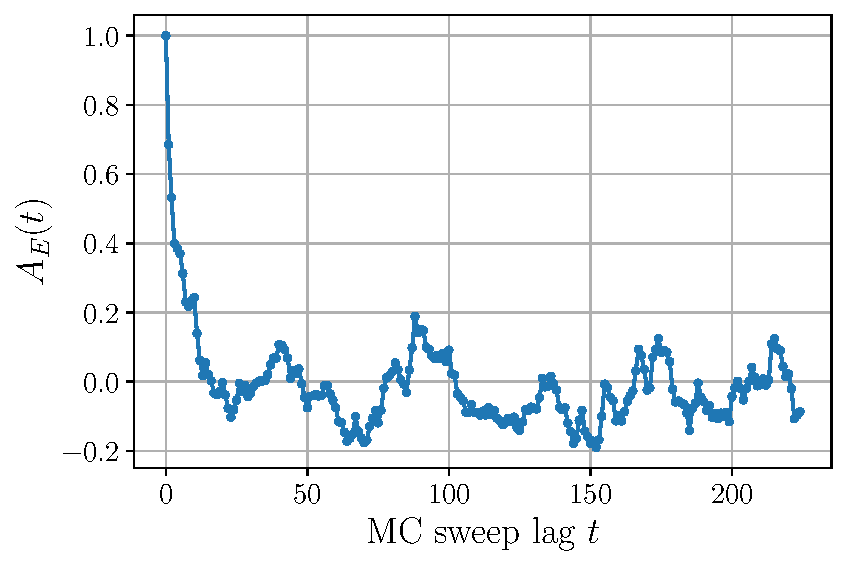
\includegraphics[width=\textwidth]{images/monte_carlo/autocorrfn.pdf}
    \end{subfigure}
    \caption{Exponential decay of energy density autocorrelation function.}
    \label{}
\end{figure}
%%% FIG %%%
\section{Estimation of expectation values and errors}
Once we have a set of uncorrelated Monte Carlo observable measurements, it is a simple task to calculate the mean and standard deviation of the uncorrelated observable measurement data $(|m|, e)$. However, for quantities that are not measured directly in the simulation but are computed as non-linear combinations of basic observables $(\chi, C_V, U_L)$, deriving a propagated error is a highly non-trivial task. Therefore, we utilize \textit{Jackknife analysis} to create large blocks/bins of the data and perform the required computations.

\subsection{Jackknife binning analysis}
We begin by binning the $N$ measurements of observable $\mathcal{O}$ into $N_B$ non-overlapping bins of length $k$ such that $N_B k = N$, and construct a shorter time series of bin averages. The bin average for the $j^\text{th}$ bin is defined as
\begin{equation}
    \mathcal{O}^{(B)}_j \equiv \frac{1}{k} \sum_{i = 0}^{k-1} \mathcal{O}_{jk+i} 
\end{equation}
Below is a visual representation of the binning process 
\begin{gather*}
    \{\underbrace{\{\mathcal{O}_0, \mathcal{O}_1 \ldots \mathcal{O}_{k-1}\}}_{\overline{\mathcal{O}}^{(B)}_0}, \underbrace{\{\mathcal{O}_{k}, \mathcal{O}_{k+1} \ldots \mathcal{O}_{2k-1}\}}_{\overline{\mathcal{O}}^{(B)}_1}, \ldots\ldots ,\underbrace{\{\mathcal{O}_{(N_B-1)k}, \mathcal{O}_{(N_B-1)k+1} \ldots \mathcal{O}_{N-1}\}}_{\overline{\mathcal{O}}^{(B)}_{N_B-1}}\} \\
    \Downarrow \\
    \{
        \overline{\mathcal{O}}^{(B)}_0, \overline{\mathcal{O}}^{(B)}_1, \overline{\mathcal{O}}^{(B)}_2 \ldots ,\overline{\mathcal{O}}^{(B)}_{N_B-1} 
    \}
\end{gather*}
Knowing the bin averages for the observables $\mathcal{O} \in \{\abs{m}, m^2, m^4, e, e^2 \}$, the bin estimates of the derived quantities are estimated as
\begin{equation}
    \chi^{(B)}_j = \beta \: L^2\:\qty(\overline{m^2}^{(B)}_j - \qty[\overline{|m|}^{(B)}_j]^2)
\end{equation}
\begin{equation}
    {C_V}^{(B)}_j = \beta ^2\: L^2 \:\qty(\overline{e^2}^{(B)}_{\:\:\:j} - \qty[\overline{e}^{(B)}_j]^2)
\end{equation}
\begin{equation}
    {U_L}^{(B)}_{\:\:\:j} = 1 - \frac{\overline{m^4}^{(B)}_j}{3\qty[\overline{m^2}^{(B)}_j]^2}
\end{equation}
% \begin{gather}
%     \chi^{(B)}_j = \beta \: L^2\:\qty(\overline{m^2}^{(B)}_j - \qty[\overline{|m|}^{(B)}_j]^2) \\[4pt] 
%     {C_V}^{(B)}_j = \beta ^2\: L^2 \:\qty(\overline{e^2}^{(B)}_{\:\:\:j} - \qty[\overline{e}^{(B)}_j]^2) \\
%     {U_L}^{(B)}_{\:\:\:j} = 1 - \frac{\overline{m^4}^{(B)}_j}{3\qty[\overline{m^2}^{(B)}_j]^2}
% \end{gather}
We denote these derived quantities by $\rho $ such that $\rho \in \{\chi , C_V, U_L\}$. The means over the bin averages (for $\mathcal{O}$) and bin estimates (for $\rho $) are also calculated
\begin{subequations}
    \begin{gather}
        \overline{\mathcal{O}} = \overline{\overline{\mathcal{O}}^{(B)}_j} = \frac{1}{N_B} \sum_{i=0}^{N_B-1} \overline{\mathcal{O}}^{(B)}_j \\
        \overline{\mathcal{\rho }} = \overline{{\rho }^{(B)}_j} = \frac{1}{N_B} \sum_{i=0}^{N_B-1} {\rho }^{(B)}_j
    \end{gather}       
    \label{binaverage} 
\end{subequations}
\!\!\!For the Jackknife error analysis, we begin by constructing the same number ($N_B$) of Jackknife bins containing all data but the $j^\text{th}$ bin of the previously mentioned binning method. The Jackknife averages for these new bins are defined as 
\begin{gather}
    \overline{\mathcal{O}}^{(J)}_j = \frac{N\overline{\mathcal{O}} - k \overline{\mathcal{O}}^{(B)}_j}{N - k} \\
    \overline{\rho }^{(J)}_j = \frac{N\overline{\rho } - k {\rho}^{(B)}_j}{N - k}
\end{gather}          
Since we are using the same data again and again while forming the Jackknife bins, these bins are trivially correlated, and as a result, the Jackknife bin variance is much smaller than is expected. This can be corrected by multiplying the sample variance by another factor of $(N_B-1)^2$ resulting in 
\begin{subequations}
    \begin{gather}
        \delta \overline{\mathcal{O}} = \sqrt{\frac{N_B-1}{N_B} \sum_{j=0}^{N_B-1}\qty(\overline{\mathcal{O}}^{(J)}_j - \overline{\mathcal{O}})^2} \\
        \delta \rho  = \sqrt{\frac{N_B-1}{N_B} \sum_{j=0}^{N_B-1}\qty(\overline{\rho }^{(J)}_j - \overline{\rho})^2}
    \end{gather}     
    \label{jackknifeerror}
\end{subequations}
\!\!\!Therefore, using the calculated values from Eq. \eqref{binaverage} and Eq. \eqref{jackknifeerror}, we get our mean and error estimates of the observable expectation values and the derived physical quantities
\[
    \text{Estimate of }\expval{\mathcal{O}} \rightarrow \overline{\mathcal{O}} \pm \delta \overline{\mathcal{O}}, \qquad\qquad \text{Estimate of }{\rho } \rightarrow \overline{\rho } \pm \delta {\rho } 
\]

\section{Critical slowing down near phase transition}
Phase transitions, in general, are associated with a discontinuity in the first derivative (for first-order phase transitions) or a divergence in the second derivative (for second-order phase transitions). For example, the classical Ising model is characterized by a second-order phase transition at a critical temperature $T_c$. Above this temperature $(T>T_c)$, the spins are randomly aligned and correspond to the \textit{paramagnetic} phase. Below this temperature $(T<T_c)$, the spins majorly align in one of the directions to form the \textit{ferromagnetic} phase of the system.
%%% FIG %%%
\begin{figure}[!htb]
    \centering
    \begin{subfigure}[b]{0.4\textwidth}  %keep total sum <1 to show in same line
        \centering
        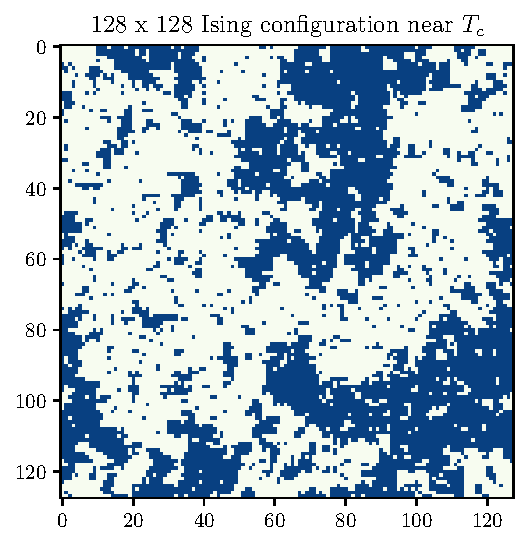
\includegraphics[width=\textwidth]{images/monte_carlo/ising_config_128.pdf}
        \caption{Domain formation near $T_c$ $(T=2.30)$.}
        \label{domain}
    \end{subfigure}
    \hspace{1em}  %\hfill
    \begin{subfigure}[b]{0.5\textwidth}
        \centering
        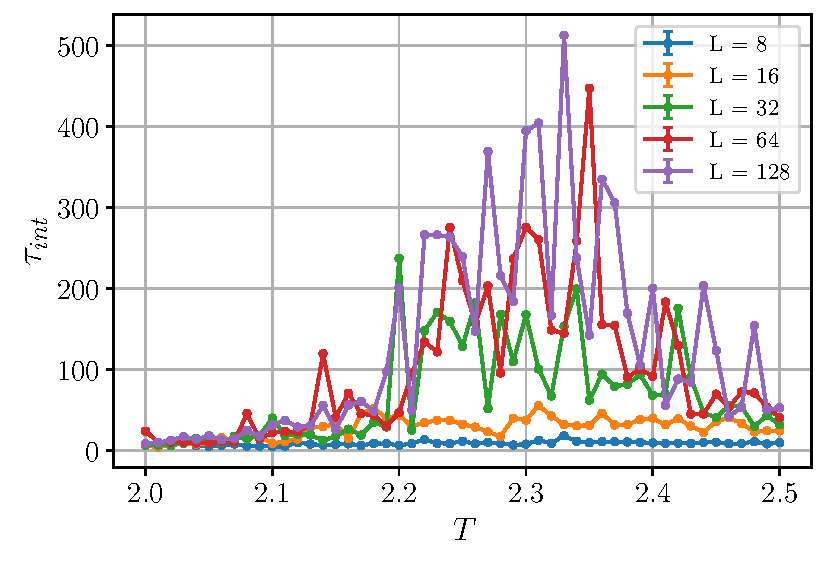
\includegraphics[width=\textwidth]{images/monte_carlo/metropolis_autocorr_time.pdf}
        \caption{High autocorrelation times near $T_c$ for Metropolis.}
        \label{autocorr_metropolis}
    \end{subfigure}
    \caption{Critical slowing down near the transition point in the Ising model.}
    \label{}
\end{figure}
%%% FIG %%%
\FloatBarrier \!\!\!\!\!\!\!\!\!
In the paramagnetic phase, at high temperatures, the spin configuration is random and there are little to no spatial correlations. However, as the temperature decreases, we enter the paramagnetic phase and spins tend to align themselves with their neighbors. As a result, we form large \textit{domains} or \textit{clusters} of spins and we have a high degree of spatial correlation (Fig. \ref{domain}), often measured by the parameter $\xi$, known as the correlation length. As one approaches the critical temperature $T_c$ from the above, the onset of strong correlations results in \textit{domain flips} which cause high fluctuations in magnetization and energy. Since the Metropolis algorithm performs local updates and the spins have a strong spatial correlation, we need to wait for a long autocorrelation time to get independent subsequent measurements (Fig. \ref{autocorr_metropolis}). This is known in literature as \textit{critical slowing down}.~\\~\\
The phenomena of critical slowing down is primarily dependent on the algorithm used. Since local update (such as Metropolis) take a long time to flip the domains and generate statistically independent configurations, they have a significantly higher computational cost as a tradeoff to their conceptual simplicity.~\\~\\
Therefore, it should be intuitively clear that some sort of non-local updates should be able to alleviate this problem by flipping entire clusters of spins. This class of algorithms is generally known as \textit{Cluster-update algorithms}. Although the critical slowing down can be significantly reduced with cluster algorithms, they are still far less general applicable than local update algorithms.

\section{Wolff Cluster algorithm}

\end{document}